\documentclass[11pt]{article}
\usepackage[margin=1in]{geometry}
\usepackage{amsmath}
\usepackage{booktabs}
\usepackage{graphicx}
\usepackage{float}
\usepackage{enumitem}
\usepackage[hidelinks]{hyperref}
\emergencystretch=3em
\graphicspath{{figs/}}

\newcommand{\code}[1]{\texttt{#1}}

\title{Postmortem: lost accelerometer samples in the October 2026 campaign}
\author{Ilan Upfal}
\date{3 November 2026}

\begin{document}
\maketitle

\noindent\fbox{\parbox{\dimexpr\textwidth-2\fboxsep-2\fboxrule\relax}{%
\textbf{Disclaimer: prepared with AI assistance.} This report, the analysis
scripts behind it and much of its text were produced with an AI assistant
(Claude, by Anthropic), working with the author. The numbers in it were
computed by scripts from the raw data and can be reproduced
(\code{reports/accel\_postmortem/make\_figures.py}), but the analysis, the
interpretation and the wording may still contain errors that neither caught.
Each finding states how certain it is; treat those marked as the best
explanation or not confirmed as hypotheses. Please check the numbers and
reasoning that matter to you, and run the checks in
Section~\ref{sec:verify}, before changing equipment, software or published
results on the strength of this report. Questions and corrections are
welcome.}}
\vspace{1em}

\section*{Summary}

\paragraph{What happened.} In every accelerometer capture of the October 2026
production campaign (6--15 October) and of the 21 October ring-down tests,
about one sample in five was lost. The sensors produce 1493 samples per second
per channel; the files contain about 1205. The losses come in a regular
pattern: 84 consecutive samples are kept, then about 19 are missing, then 84
are kept, and so on.

\paragraph{Effect.} The vibration levels (variances) used to find the
vibration regions and to build the design-space maps are not affected. The
frequency content is affected: analyses that assumed evenly spaced samples
put every frequency about 19\% too low, and even with the correct handling
each spectrum carries weak copies of every peak $\pm$14\,Hz to either side.
All of this can be handled in the analysis, so the existing data remain
usable.

\paragraph{Cause.} The accelerometer board, its firmware and the RS-485 link
can deliver all the data; the vendor showed this with the same settings. The
loss happens because our acquisition software on the lab PC reads too slowly:
each read takes 69\,ms on average, while the board fills a maximum-size read
(84 samples) in 56\,ms. The most likely reasons are a USB setting that our
code tries to change but silently cannot on Windows, and competition for the
processor from the live plot and the load-cell reader running in the same
program.

\paragraph{What we ask.} Two quick checks on the acquisition PC
(Section~\ref{sec:verify}), then, before the next campaign, one setting
change on the PC and a few changes to the acquisition software, ending with
an acceptance test (Section~\ref{sec:fix}).

%======================================================================
\section{Background}
%======================================================================

The AF10R1 board carries four LIS2DS12 accelerometers (S1 at the blade root
to S4 at the tip), each sampling three axes. A sample-set is one reading of
all 12 channels (24 bytes). The board stores sample-sets in a buffer, and the
PC collects them over RS-485 with Modbus at 921\,600 baud. The capture loop
in \code{main.py} repeats:
\begin{enumerate}[nosep]
  \item ask the board how many sample-sets are waiting (register AVAIL);
  \item read $\min(\text{AVAIL}, 84)$ sample-sets in one bulk read;
  \item write them to the CSV file, all with the time the read finished.
\end{enumerate}
The firmware limits one bulk read to 84 sample-sets (AF10R1 User Guide,
Section~4: ``Max FC04 1008 registers''). The limit is compiled into the
vendor firmware, of which we have only the binaries.

The problem was first noticed when tip-flick ring-downs gave a first flap
mode of 47.5\,Hz while a 4000\,fps high-speed video of a flapwise ring-down
of the same blade gave 62.7\,Hz (Section~\ref{sec:where},
Figure~\ref{fig:evidence}).

%======================================================================
\section{Diagnosis}
%======================================================================

We state for each finding what the evidence is and how certain it is. All
numbers in Sections~\ref{sec:loss}--\ref{sec:where} are computed from the raw
data, by \code{reports/accel\_postmortem/make\_figures.py}: all 1342
production captures (1.15 million reads), the 121 ring-down captures and the
high-speed video.

\subsection{The sensors sample at 1493 Hz}

The board is configured for 1600\,Hz, but the sensors run on an internal
oscillator. The vendor measured 1493\,Hz over a 5-minute test, stable to
$\pm$1\,Hz on all four sensors (User Guide, Section~5.1). Our data agree:
with this rate, the first flap mode measured by the accelerometer matches the
high-speed video to 0.2\,Hz (Section~\ref{sec:where}). All numbers below use
1493\,Hz.

\textit{Certainty: measured by the vendor, consistent with our data.}

\subsection{Every read is full, and samples are lost}
\label{sec:loss}

\begin{figure}[H]
  \centering
  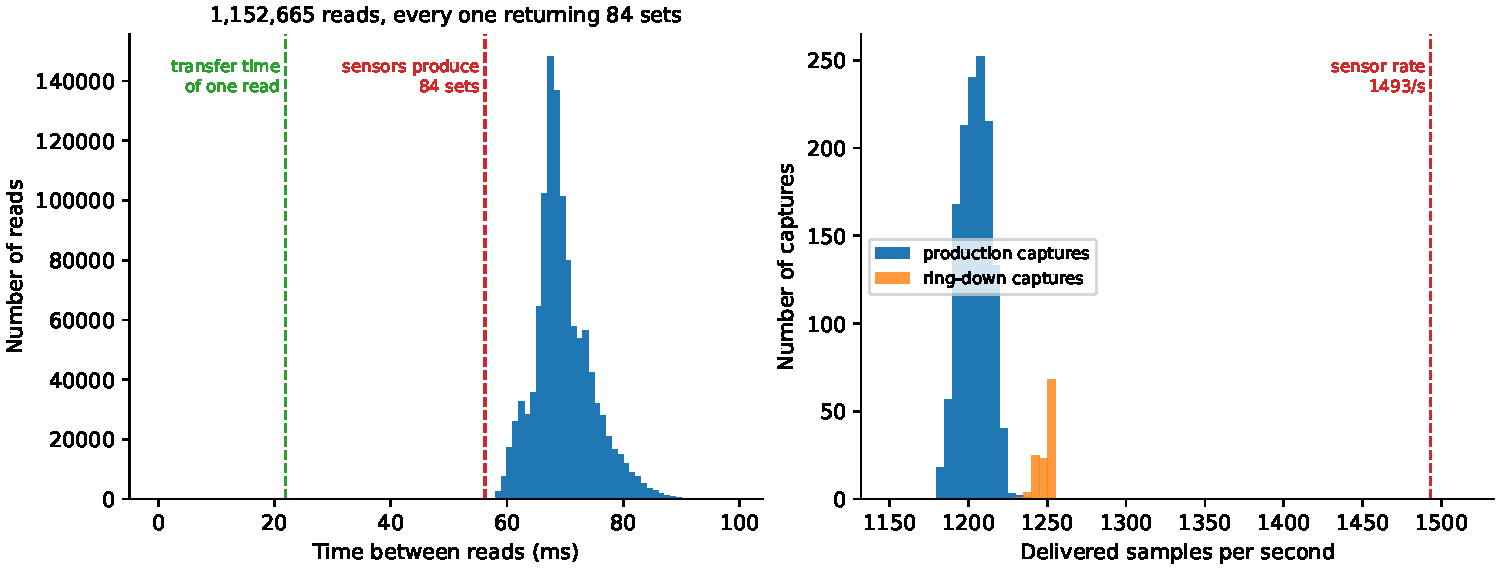
\includegraphics[width=\textwidth]{read_cycle.pdf}
  \caption{Left: time between consecutive reads in the production captures.
  Every one of these reads returned the maximum of 84 sample-sets. The
  sensors produce 84 sets in 56\,ms (red), and sending them takes 22\,ms
  (green); the reads come every 69\,ms. Right: delivered sample-sets per
  second for each capture, against the sensor rate of 1493 per second.}
  \label{fig:cycle}
\end{figure}

\begin{table}[H]
  \centering
  \begin{tabular}{lcc}
    \toprule
    & Production (32 runs) & Ring-downs (2 runs) \\
    \midrule
    Captures / reads examined & 1342 / 1\,152\,665 & 121 / 17\,784 \\
    Reads returning exactly 84 sets & 100\% & 100\% \\
    Time between reads, median (5--95\%) & 68.8\,ms (62.1--79.3) & 67.0\,ms (66.1--68.7) \\
    Sets produced per read cycle & 102.7 & 100.0 \\
    Delivered rate, median & 1205 per s & 1250 per s \\
    Samples lost & 19.3\% & 16.2\% \\
    \bottomrule
  \end{tabular}
  \caption{Read statistics from the raw files.}
  \label{tab:reads}
\end{table}

Two facts settle that samples are lost (Table~\ref{tab:reads},
Figure~\ref{fig:cycle}):
\begin{itemize}
  \item \textbf{Every read returned the maximum.} Not one of 1.15 million
        reads returned fewer than 84 sets, so at every read at least 84 sets
        were waiting: the software never caught up with the sensors.
  \item \textbf{Too few samples arrive.} Between two reads (69\,ms) the
        sensors produce about 103 sets; 84 are kept. The files hold 1205 sets
        per second instead of 1493.
\end{itemize}
If the board had kept the unread sets in its 1024-set buffer, the reads would
have fallen further behind but lost nothing until the buffer overflowed,
about 4\,s into each capture. The phase test in Section~\ref{sec:where}
(Table~\ref{tab:phase}) shows samples already missing within the first 4\,s,
so the excess was lost from the start. The most likely explanation is that the
board discards whatever a read does not return. This could be confirmed from
the board's OVERRUN and COUNTER registers, which we did not log.

\textit{Certainty: the loss and its size are measured directly. That the board
discards unreturned sets is the best explanation but is not confirmed.}

\subsection{The samples are lost between reads, not within them}
\label{sec:where}

The 84 sets of one read are consecutive sensor samples; the gap falls between
reads. Three independent checks on the 30 flapwise tip-flick ring-downs
of 21 October (tip sensor, flapwise axis) support this.

\begin{figure}[H]
  \centering
  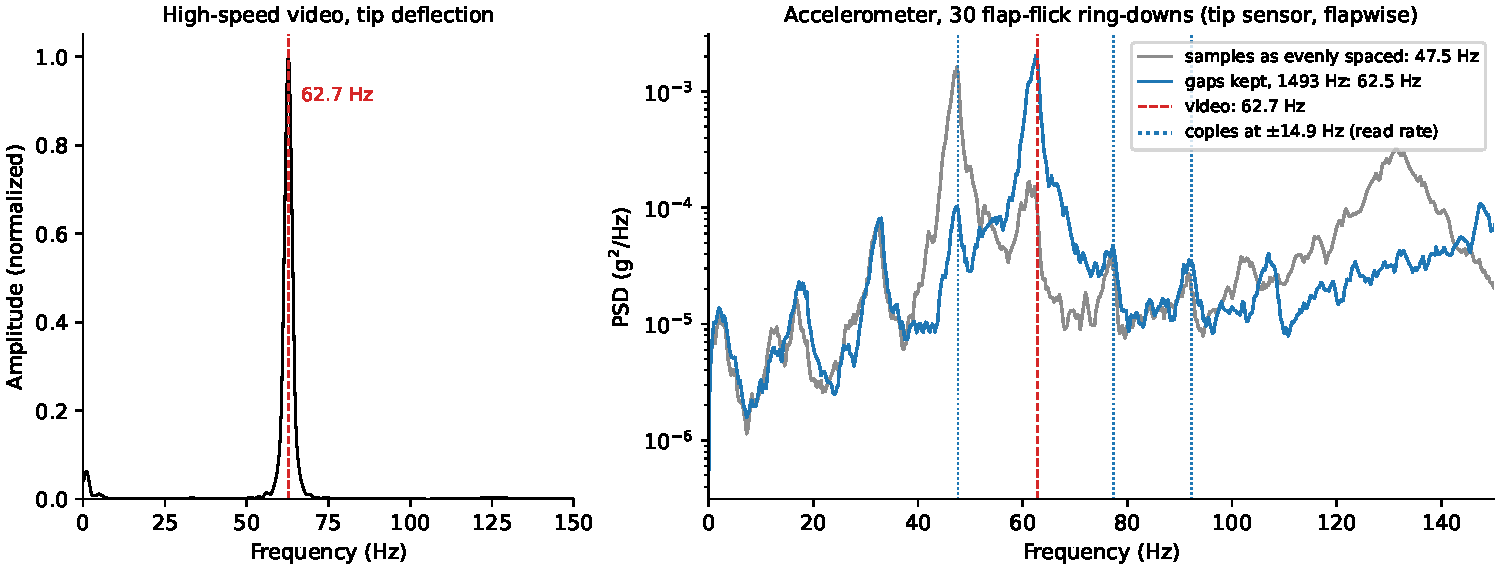
\includegraphics[width=\textwidth]{evidence.pdf}
  \caption{Left: spectrum of the blade tip deflection tracked in a 4000\,fps
  high-speed video of a flapwise ring-down. Right: median accelerometer
  spectrum of the 30 flapwise ring-downs, computed two ways. Grey: samples
  treated as evenly spaced at the delivered rate (the method used before the
  problem was found). Blue: each read's 84 samples placed consecutively at
  1493\,Hz with the missing samples left as gaps. Red dashed: the video
  frequency. Blue dotted: where the gaps should create copies of the mode.}
  \label{fig:evidence}
\end{figure}

\begin{enumerate}
  \item \textbf{High-speed video.} The video gives the first flap mode at
        62.7\,Hz (Figure~\ref{fig:evidence}, left). Treating the
        accelerometer samples as evenly spaced puts it at 47.5\,Hz, 24\%
        low. Placing each read's 84 samples consecutively at 1493\,Hz and
        leaving the missing samples as gaps puts it at 62.5\,Hz, 0.2\,Hz
        from the video (right). Only the second picture is consistent with
        the video.
  \item \textbf{Predicted copy peaks.} If the gaps repeat with every read,
        every peak must have weak copies at $\pm$ the read rate (14.9\,Hz for
        these captures). They appear exactly there: at 47.6\,Hz, 77.4\,Hz and
        92.2\,Hz ($62.5 - 14.9$, $62.5 + 14.9$ and $62.5 + 2\times14.9$),
        with 5.1\%, 2.3\% and 1.7\% of the mode's power. (The grey curve's
        47.5\,Hz peak is not this copy: there the whole mode has been
        shifted.)
  \item \textbf{Phase from read to read.} Within each read, the phase of the
        62.7\,Hz vibration can be measured. From one read to the next it must
        advance by a fixed amount: by the 84 samples of one read
        ($-2.95$\,rad, wrapped) if the reads are continuous, or by the 67\,ms
        between reads ($+1.28$\,rad) if samples are missing between them.
        Table~\ref{tab:phase} shows the measured advance.
\end{enumerate}

\begin{table}[H]
  \centering
  \begin{tabular}{lcc}
    \toprule
    & Read pairs & Phase change per read \\
    \midrule
    Expected if reads are continuous & & $-2.95$\,rad \\
    Expected if 67\,ms passes between reads & & $+1.28$\,rad \\
    Measured, first 4\,s of the capture & 43 & $+1.18$\,rad \\
    Measured, 4--6\,s & 74 & $+1.09$\,rad \\
    \bottomrule
  \end{tabular}
  \caption{Phase change of the 62.7\,Hz flap mode between consecutive reads,
  30 flapwise ring-downs (only reads where the mode is ringing; most flicks
  start 3--4.5\,s into the capture).}
  \label{tab:phase}
\end{table}

\textit{Certainty: high; three independent checks agree.}

\subsection{The board and the link are not the bottleneck}

\begin{itemize}
  \item The vendor streamed for 5 minutes with the same firmware, the same
        84-set limit and the same baud rate, and received 448\,517 sets (1493
        per second) with no overruns and no errors (User Guide, Section~5.1).
  \item At the full sensor rate the data need 35.8\,kB/s; the link carries
        92.2\,kB/s, so it is 39\% loaded.
  \item Sending one full 84-set read takes 21.9\,ms, well under the 56.3\,ms
        the sensors need to fill it.
\end{itemize}
So the 84-set limit is not the problem, and raising it would not help. A
loop that reads at least every 56\,ms never finds more than 84 sets waiting.

\textit{Certainty: high.}

\subsection{The cause is the acquisition software on the lab PC}

Of each 69\,ms read cycle, 22\,ms is the data transfer and about 47\,ms is
spent on the PC. Reading the acquisition code, we find four contributors:

\begin{enumerate}
  \item \textbf{USB latency timer not lowered.} The USB-to-RS-485 adapter
        holds incoming bytes for up to 16\,ms by default before passing them
        on. The vendor guide says to set this to 1\,ms, and \code{main.py}
        tries to (\code{set\_low\_latency}), but that function only works on
        Linux. The lab PC runs Windows (ports \code{COM11}/\code{COM12}), so
        the call fails, and the failure is not reported. Each read cycle has
        two exchanges with the board (AVAIL, then the bulk read), so this can
        add up to about 30\,ms per cycle.
  \item \textbf{Competing work in the same program.} During production
        captures the read loop runs in a background thread while the main
        thread services the live plot continuously, with no pause, and a
        third thread reads the load cell. Python runs only one thread at a
        time, so these slow the read loop. Consistent with this, production
        reads are both slower and far more irregular (62--79\,ms) than the
        ring-down reads (66--69\,ms).
  \item \textbf{Two exchanges per read.} Asking for AVAIL before every bulk
        read doubles the number of round trips.
  \item \textbf{Writing each row to the CSV during the capture.} 84 file
        writes per read inside the time-critical loop.
\end{enumerate}

\textit{Certainty: that the PC side is too slow is measured. Which of the
four contributors dominates is not; the checks in
Section~\ref{sec:verify} will show it.}

%======================================================================
\section{Analysing the existing data}
%======================================================================

The existing data remain usable. What needs care depends on the quantity.

\begin{table}[H]
  \centering
  \begin{tabular}{p{4.6cm}p{2.4cm}p{7.2cm}}
    \toprule
    Quantity & Affected? & What to do \\
    \midrule
    Variance, RMS, normalized variance; vibration regions; design-space
    maps & No &
    Use as is. 81\% of the samples, lost in a regular pattern unrelated to
    the blade motion, give the same variance with slightly less precision. \\
    \addlinespace
    Peak acceleration, clipping & No & Use as is. \\
    \addlinespace
    Load cell & No & Separate data acquisition, not affected. \\
    \addlinespace
    Spectra and frequencies & Yes &
    Place each read's samples consecutively at 1493\,Hz and leave the gaps
    empty (the ``gap-aware'' method, below). Never treat the samples as
    evenly spaced. \\
    \addlinespace
    Weak spectral peaks & Yes &
    Ignore peaks at $\pm$14--15\,Hz (and multiples) from a stronger peak:
    they are copies created by the gaps. \\
    \addlinespace
    Frequencies above 150\,Hz & Partly &
    Quote with $\pm$15\,Hz: they depend on the exact sample rate, which is
    known only from the vendor's measurement. \\
    \addlinespace
    Time-domain fits (damping, zero crossings, filtering), accelerometer--load
    cell phase & Yes &
    Use the gap-aware time base, and fit only within a read (84 samples,
    56\,ms) or with methods that tolerate gaps. \\
    \bottomrule
  \end{tabular}
  \caption{Effect of the lost samples on each kind of result.}
  \label{tab:impact}
\end{table}

\paragraph{The gap-aware method.} For each capture: (1)~group the rows by
their read time (the \code{time} column, shared by the 84 rows of one read);
(2)~give the rows of each read consecutive slots on a grid of spacing
$1/1493$\,s, ending at the read time; (3)~leave the grid slots between reads
empty; (4)~compute spectra with Welch's method, ignoring the empty slots. The
functions \code{batch\_grid}, \code{gridded} and \code{masked\_welch} in
\code{scripts/data\_analysis/accel\_spectra.py} do this, and
\code{drop\_sidebands} removes the copy peaks from a list of peaks. The
summary pipeline (\code{extract\_run\_summary.py}, version 1.4 or later) uses
them for every spectrum it stores, and the blue curve in
Figure~\ref{fig:evidence} is computed this way.

\paragraph{Results to redo.} Any spectrum computed before 29 October with
evenly spaced samples has frequencies 16--19\% too low (the delivered rate
divided by 1493). Any computed with the gap-aware method at 1600\,Hz has
its higher peaks (above $\sim$100\,Hz) up to about 7\% (one copy spacing,
$\sim$15\,Hz) too high; sharp low-frequency peaks are unaffected. Variance-based results do
not need to be redone.

%======================================================================
\section{Checks on the acquisition PC}
\label{sec:verify}
%======================================================================

These two checks take about 15 minutes and confirm the diagnosis before any
code is changed. Both use the vendor's streaming script with the board alone,
no motor and no load cell.

\begin{enumerate}
  \item \textbf{As configured now.} From \code{scripts/aquire\_data}, run
        \begin{center}\small\code{python test\_modbus.py COM12 stream test\_default.csv}\end{center}
        let it stream for 60\,s, then stop it with Ctrl+C. Record the
        delivered rate and the overrun count it prints.
  \item \textbf{With the latency timer at 1\,ms.} In Windows Device Manager,
        open the USB serial adapter for COM12, then Port Settings $\to$
        Advanced, set \emph{Latency Timer (msec)} to 1, reconnect, and repeat
        the 60\,s stream.
\end{enumerate}

\begin{table}[H]
  \centering
  \begin{tabular}{p{5.5cm}p{9cm}}
    \toprule
    Result & Meaning \\
    \midrule
    Check 1 $\approx$1250/s, check 2 $\approx$1493/s & The USB latency
    timer is the main cause. Keep it at 1\,ms; the code changes below are
    still recommended. \\
    \addlinespace
    Both $\approx$1493/s & The board and PC are fine on their own; the
    loss comes from the extra work in \code{main.py} (live plot, load-cell
    thread, per-row writes). \\
    \addlinespace
    Both $\approx$1250/s & Something else on the PC limits the loop (USB
    adapter, drivers); compare with a Linux machine. \\
    \bottomrule
  \end{tabular}
  \caption{How to read the two checks. 1493/s with no overruns matches the
  vendor's test.}
\end{table}

%======================================================================
\section{Fixing the acquisition}
\label{sec:fix}
%======================================================================

In order of priority:

\begin{enumerate}
  \item \textbf{Set the USB latency timer to 1\,ms} on the acquisition PC,
        as in check~2. It is a one-time setting per adapter, but it is lost
        if the adapter moves to another USB port, so it belongs on the
        pre-run checklist.
  \item \textbf{Make the latency setting visible in the code.}
        \code{set\_low\_latency} should report when it fails, and on Windows
        print the Device Manager instructions, so this cannot fail silently
        again.
  \item \textbf{Log the board's counters on every read.} Write AVAIL,
        OVERRUN and the board's sample COUNTER into the capture file with
        each read. A capture is then complete only if COUNTER advances by
        exactly the number of rows written, OVERRUN stays 0 and AVAIL stays
        below 84. This proves each capture is gap-free, and COUNTER over the
        capture time gives each board's actual sample rate, instead of
        relying on the vendor's value.
  \item \textbf{Keep the read loop free of other work.} Collect the rows in
        memory and write the file after the capture; stop servicing the live
        plot during the capture, or update it only between angles; give the
        main thread a short sleep while waiting for the capture threads.
  \item \textbf{Read before 84 sets accumulate.} Aim for a read every
        20--40\,ms (30--60 sets per read), so AVAIL never reaches 84 even
        when the PC is briefly busy.
  \item \textbf{Fallback: lower the sample rate.} If the loop still cannot
        keep up, 800\,Hz halves the data rate. It still resolves frequencies
        up to 400\,Hz, above every peak of interest found so far
        ($\leq$300\,Hz).
  \item \textbf{Ask InUnit} to confirm what the board does when more than 84
        sets are waiting, and the actual buffer size in the current firmware.
\end{enumerate}

\paragraph{Acceptance test before the next campaign.} A 60\,s capture with
the full setup (motor, load cell, live plot as it will be used) must deliver
1493\,$\pm$\,5 sets per second, OVERRUN = 0, and COUNTER increments equal to
the rows written.

%======================================================================
\section*{References}
%======================================================================

\begin{itemize}[nosep]
  \item InUnit AB, \emph{AF10R1 User Guide}, DOC-2026-06-12-01 rev v1 (draft),\\
        \code{data/pcb\_documentation/AF10R1\_UG.pdf}.
  \item \code{reports/accel\_postmortem/make\_figures.py} (analysis
        repository): computes every number, table and figure in this report
        from the raw data.
\end{itemize}

\end{document}
